A modificação, de forma controlada, no comportamento de um sistema, 
garantindo uma maior eficiência é o objetivo do controle de sistemas,
que é estudado desde os antigos, mas que obteve grande relevância na necessidade trazida com a revolução industrial, 
e hoje conta com o seu segmento específico da engenharia, com diversos trabalhos nessa área e uma infinidade de aplicações. 
 

A principal tarefa de um engenheiro é, segundo \citeauthor{dorf2011modern}(\citeyear{dorf2011modern}), 
"o processo de concepção ou invenção de formas, partes e detalhes de um sistema para alcançar um propósito específico", 
processo este que soma a grande capacidade de análise e a criatividade para atender as demandas da função, 
como é o caso de projeto em engenharia no segmento de Sistemas de Controle, 
cujo objetivo é obter a configuração, as especificações e a identificação de processos para atender uma necessidade real. 


Uma concepção semelhante é trazida por \citeauthor{nise2009engenharia}(\citeyear{nise2009engenharia}) onde "Um sistema de controle consiste em subsistemas e processos(ou plantas) construídos com o objetivo de se obter uma saída desejada com desempenho desejado para uma entrada específica fornecida".


Os sistemas de controle atuam basicamente gerando respostas específicas para estímulos específicos de forma controlada e automática, 
trazendo vantagens nas aplicações em diversas áreas, tais como, 
na movimentação de grandes equipamentos com precisão, 
em locais remotos ou perigosos, 
na compensação de perturbações, 
manipulando os dados de forma conveniente.





%%%%%%%%%%%%%%%%%%%%%%%%%%%%%%%%%%%%%%%%%%%%%%%%%%%%%%%%%%%%
\section{Diagrama de Blocos}
%%%%%%%%%%%%%%%%%%%%%%%%%%%%%%%%%%%%%%%%%%%%%%%%%%%%%%%%%%%%



Os sistemas de controle são geralmente representados através de diagramas de blocos ou fluxo de sinais, 
como na Figura \ref{fig:processo}, 
convenientes ao seu desenvolvimento e análise. 
É composto por uma caixa representando o sistema a ser controlado, 
setas no sentido da caixa representando as entradas do processo e setas no sentido para fora da caixa para indicar a saída do sistema.


Em um sistema real podem haver muitas variáveis de entrada e de saída, 
mas a abordagem clássica de controle isola apenas uma das variáveis de entrada e uma de saída, 
ficando o sistema conhecido pela sigla em inglês SISO (\emph{Single In Single Out} - Única Entrada e Única Saída).


\begin{figure}[!htb]
\centering
\caption{ Diagrama de blocos de sistema de controle}
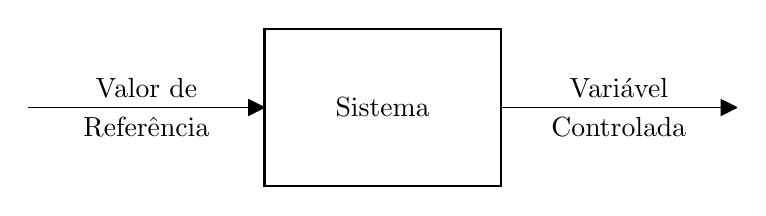
\begin{tikzpicture}[scale=1]
%\draw [lightgray](0,0) grid (9,2);
\draw (0,1) -- (3,1);
\draw [black, thick](3,0) rectangle (6, 2) ; 
\draw (6,1) -- (9,1);
\draw [fill](3,1) -- (2.8, 1.1) -- (2.8,0.9) -- (3,1);
\draw [fill](9,1) -- (8.8, 1.1) -- (8.8,0.9) -- (9,1);
\node at (4.5, 1){Sistema};
\node [above] at (1.5,1){Valor de};
\node [below] at (1.5,1){Referência};
\node [above] at (7.5,1){Variável};
\node [below] at (7.5,1){Controlada};
\end{tikzpicture}
\label{fig:processo}

{\small Fonte: \cite{Ogata} }
\end{figure}


O diagrama de blocos mostrado na Figura \ref{fig:processo} é uma simplificação ao máximo de um sistema de controle, 
contém apenas o bloco representando o sistema, 
uma entrada, para o valor de referência, 
e uma saída com o valor da variável controlada.


Em \citeauthor{Ogata}(\citeyear{Ogata}) % - Capítulo 3.3 - 
são encontradas definições, 
comentários sobre vantagens, 
aplicações e procedimento para construção de Diagramas de blocos, 
assim como a representação de sistemas em malha aberta, 
malha fechada, 
perturbações, 
técnicas e regras da álgebra de blocos.





O diagrama de blocos mostrado na Figura \ref{fig:processo} é uma simplificação ao máximo de um sistema de controle, contém apenas o bloco representando o sistema, uma entrada, para o valor de referência, e uma saída com o valor da variável controlada. A Figura \ref{fig:malhaAberta}, divide os bloco do sistema em dois: controlador e planta. Neste caso, um sistema de controle em malha aberta, ou seja, não há uma reinserção do sinal de saída à entrada, chamada de realimentação ou retroalimentação. Assim, a entrada possui o valor de resposta desejada, que alimenta o processo e a saída apresenta a resposta real, porém nada garante que a resposta real está coerente ao valor de entrada.

\begin{figure}[!htb]
\centering
\caption{ Diagrama de blocos de sistema de controle em malha aberta}
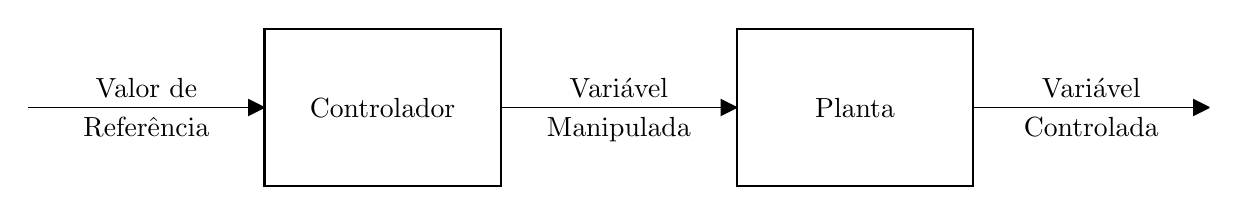
\begin{tikzpicture}[scale=1]
%\draw [lightgray](0,0) grid (15,2);
\draw (0,1) -- (3,1);
\draw [black, thick](3,0) rectangle (6, 2) ; 
\draw (6,1) -- (9,1);
\draw [black, thick](9,0) rectangle (12, 2) ; 
\draw (12,1) -- (15,1);

\draw [fill]( 3,1) -- ( 2.8, 1.1) -- ( 2.8,0.9) -- ( 3,1);
\draw [fill]( 9,1) -- ( 8.8, 1.1) -- ( 8.8,0.9) -- ( 9,1);
\draw [fill](15,1) -- (14.8, 1.1) -- (14.8,0.9) -- (15,1);

\node at ( 4.5, 1){Controlador};
\node at (10.5, 1){Planta};
\node [above] at ( 1.5,1){Valor de};
\node [below] at ( 1.5,1){Referência};
\node [above] at ( 7.5,1){Variável};
\node [below] at ( 7.5,1){Manipulada};
\node [above] at (13.5,1){Variável};
\node [below] at (13.5,1){Controlada};
\end{tikzpicture}
\label{fig:malhaAberta}

{\small Fonte: \cite{Ogata}}
\end{figure}

O diagrama da Figura \ref{fig:malhaFechada} 
apresenta realimentação, ou seja, 
uma amostra da resposta real é lida por um elemento sensor e é 
reinserida à entrada da malha, 
aonde é realizada a comparação entre resposta real e desejada, 
a diferença entre ambos os valores é chamado de Erro do Sistema e é 
baseado nesse valor que o controlador tem condições de efetuar as 
devidas correções, geralmente, 
afim de manter o sistema estável no valor de resposta desejada.

\begin{figure}[!htb]
\centering
\caption{ Diagrama em blocos de sistema de controle em malha fechada}
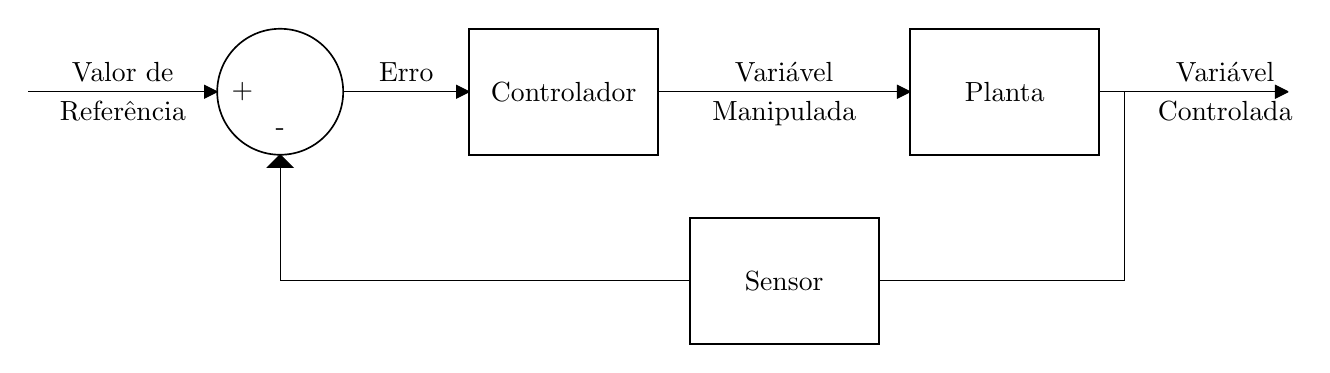
\begin{tikzpicture}[scale=0.8]
%\draw [lightgray](-3,0) grid (17, 2);
%\draw [lightgray](-3,0) grid (17,-3);
%\draw [semithick,red] (0,0) circle (0.1);

\draw (-3,1) -- (0,1);
\draw [fill]( 0,1) -- (-0.2, 1.1) -- ( -0.2,0.9) -- (0,1);
\draw [semithick,black] (1,1) circle (1.0); % Somador
\draw (2.0,1) -- (4,1);
\draw [fill]( 4,1) -- ( 3.8, 1.1) -- ( 3.8,0.9) -- ( 4,1);
\draw [black, thick](4,0) rectangle (7, 2) ; % Controlador 
\draw (7,1) -- (11,1);
\draw [fill]( 11,1) -- (10.8, 1.1) -- (10.8,0.9) -- (11,1);
\draw [black, thick](11,0) rectangle (14, 2) ; % Planta
\draw (14,1) -- (17,1);
\draw [fill](17,1) -- (16.8, 1.1) -- (16.8,0.9) -- (17,1);

\draw [black, thick](7.5,-1) rectangle (10.5, -3) ; % Sensor
\draw (14.4, 1) -- (14.4, -2) -- (10.5,-2);
\draw ( 7.5,-2) -- ( 1, -2) -- (1,0);
\draw [fill](1,0) -- (1.2,-0.2) -- (0.8,-0.2) -- (1,0);

\node [above] at (-1.5,1){Valor de};
\node [below] at (-1.5,1){Referência};
\node at (0.4,1){+};
\node at (1,0.4){-};
\node [above] at (3.0,1){Erro};
\node at ( 5.5, 1){Controlador};
\node [above] at (9.0,1){Variável};
\node [below] at (9.0,1){Manipulada};
\node at (12.5, 1){Planta};
\node [above] at (16.0,1){Variável};
\node [below] at (16.0,1){Controlada};
\node at ( 9.0,-2){Sensor};

\end{tikzpicture}
\label{fig:malhaFechada}

{\small Fonte: \cite{Ogata}}
\end{figure}


Como notação para os elementos do diagrama de blocos, 
são adotadas letras para representar matematicamente as relações entre 
as grandezas conforme Figura \ref{fig:malhaFechadaLetras}


\begin{figure}[!htb]
\centering
\caption{ Diagrama em blocos de sistema de controle em malha fechada utilizando notação matemática}
\begin{tikzpicture}[scale=0.8]
%\draw [lightgray](-3,0) grid (17, 2);
%\draw [lightgray](-3,0) grid (17,-3);
%\draw [semithick,red] (0,0) circle (0.1);

\draw (-3,1) -- (0,1);
\draw [fill]( 0,1) -- (-0.2, 1.1) -- ( -0.2,0.9) -- (0,1);
\draw [semithick,black] (1,1) circle (1.0); % Somador
\draw (2.0,1) -- (4,1);
\draw [fill]( 4,1) -- ( 3.8, 1.1) -- ( 3.8,0.9) -- ( 4,1);
\draw [black, thick](4,0) rectangle (7, 2) ; % Controlador 
\draw (7,1) -- (11,1);
\draw [fill]( 11,1) -- (10.8, 1.1) -- (10.8,0.9) -- (11,1);
\draw [black, thick](11,0) rectangle (14, 2) ; % Planta
\draw (14,1) -- (17,1);
\draw [fill](17,1) -- (16.8, 1.1) -- (16.8,0.9) -- (17,1);

\draw [black, thick](7.5,-1) rectangle (10.5, -3) ; % Sensor
\draw (14.4, 1) -- (14.4, -2) -- (10.5,-2);
\draw ( 7.5,-2) -- ( 1, -2) -- (1,0);
\draw [fill](1,0) -- (1.2,-0.2) -- (0.8,-0.2) -- (1,0);

\node [above] at (-1.5,1){r(t)};
\node at (0.4,1){+};
\node at (1,0.4){-};
\node [above] at (3.0,1){e(t)};
\node at ( 5.5, 1){f(t)};
\node [above] at (9.0,1){u(t)};
\node at (12.5, 1){g(t)};
\node [above] at (16.0,1){c(t)};
\node at ( 9.0,-2){h(t)};

\end{tikzpicture}
\label{fig:malhaFechadaLetras}

{\small Fonte: \cite{Ogata}}
\end{figure}


\nomenclature{r(t)}{Valor de Referência em função do tempo}%
\nomenclature{e(t)}{Erro em função do tempo}%
\nomenclature{f(t)}{Modelo do Controlador em função do tempo}%
\nomenclature{u(t)}{Variável manipulada}%
\nomenclature{g(t)}{Modelo da Planta do sistema}%
\nomenclature{c(t)}{Variável Controlada}%
\nomenclature{h(t)}{Modelo do elemento sensor}%

%%%%%%%%%%%%%%%%%%%%%%%%%%%%%%%%%%%%%%%%%%%%%%%%%%%%%%%%%%%%
\section{Controle Clássico}
%%%%%%%%%%%%%%%%%%%%%%%%%%%%%%%%%%%%%%%%%%%%%%%%%%%%%%%%%%%%

Os sistemas de controle clássicos possuem a predileção por tratar 
sistemas monovariáveis, lineares e invariantes no tempo, 
mas esta não é a condição mais provável para um sistema físico. 
Ao longo do tempo foram desenvolvidas ferramentas, 
como a Transformada de Laplace, 
para contornar algumas dificuldades inerentes ao equacionamento dos 
modelos matemáticos e também métodos como o dos lugares das raízes ou 
resposta de frequência.

Os sistemas de controle modernos possuem o índice de 
desempenho em termos de variáveis de estado, 
e possuem técnicas para tratar sistemas multivariáveis, 
não lineares e variantes no tempo.

A forma prática de trabalhar com sistemas de controle clássicos é 
através de modelos matemáticos para descrever a dinâmica dos sistemas 
a partir das leis físicas que regem seus comportamento e desempenho.
As variáveis dos sistemas articulam-se dinamicamente e são 
expressas matematicamente utilizando, geralmente, 
equações diferencias, e podem ser relações lineares ou não lineares. 
Para sistemas não lineares é habitual que seja feita a 
linearização do sistema, ou de uma região que se queira controlar, 
utilizando como ferramenta a Série de Taylor. 

Outra ferramenta extremamente importante é a Transformada de Laplace que 
converte uma equação diferencial no domínio do tempo em uma 
equação algébrica no domínio da frequência, 
facilitando a manipulação matemática na utilização dos métodos de controle. 

A relação das variáveis de saída com a de entrada do sistema, 
é denominada de Função de Transferência(FT) 
\nomenclature{FT}{Função de Transferência}%
e apresenta as características dinâmicas do sistema.



%%%%%%%%%%%%%%%%%%%%%%%%%%%%%%%%%%%%%%%%%%%%%%%%%%%%%%%%%%%
\subsection{Modelagem matemática}
%%%%%%%%%%%%%%%%%%%%%%%%%%%%%%%%%%%%%%%%%%%%%%%%%%%%%%%%%%%

A maioria dos sitemas físicos pode ser modelado matematicamente através de 
equações diferenciais parciais e é comum que os sistemas apresentem 
comportamento exponencial, e também apresentam não linearidades, 
que dependendo da aplicação, podem ser aproximadas em 
regiões específicas de operação e as equações sofrem 
transformadas para simplificar a manipulação e resolução dos 
problemas encontrados nos diversos sistemas assim como o 
apresentado neste estudo.


%%%%%%%%%%%%%%%%%%%%%%%%%%%%%%%%%%%%%%%%%%%%%%%%%%%%%%%%%%%
\subsection{Sistema Linear}
%%%%%%%%%%%%%%%%%%%%%%%%%%%%%%%%%%%%%%%%%%%%%%%%%%%%%%%%%%%

Quase que a totalidade dos processos naturais apresentam 
aspectos não lineares, porém a técnica de controle clássico trabalha 
apenas com sistemas lineares, assim exitem duas opções para trabalhar 
com sistemas não lineares: 
mudar o método de controle para uma ténica não convencional ou 
linearizar em torno de um ponto de operação. 
A linearização é o processo de encontrar um modelo linear que 
atenda bem a aproximação do modelo não linear em questão \cite{Ogata}.

%Lyapunov ??? provou que em uma região próxima ao ponto de operação um sistema não linear pode ser estável.

Dado um sistema \emph{S(t)} para uma entrada $u(t) = u_1(t)$ tem-se uma saída $y(t) = y_1(t)$ e para uma entrada $u(t) = u_2(t)$ tem-se uma saída $y(t) = y_2(t)$.

\begin{figure}[!htb]
\centering
\caption{ Sistema simples}
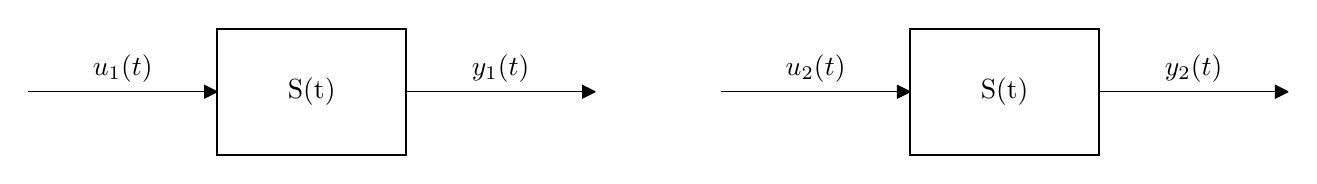
\begin{tikzpicture}[scale=0.8]
%\draw [lightgray](0,0) grid (20, 2);

\draw (0,1) -- (3,1);
\draw [fill]( 3,1) -- ( 2.8, 1.1) -- ( 2.8,0.9) -- ( 3,1);
\draw [black, thick](3,0) rectangle (6, 2) ; % S1 
\draw (6,1) -- (9,1);
\draw [fill]( 9,1) -- (8.8, 1.1) -- (8.8,0.9) -- (9,1);

\draw (11,1) -- (14,1);
\draw [fill]( 14,1) -- ( 13.8, 1.1) -- ( 13.8,0.9) -- ( 14,1);
\draw [black, thick](14,0) rectangle (17, 2) ; % S2
\draw (17,1) -- (20,1);
\draw [fill]( 20,1) -- (19.8, 1.1) -- (19.8,0.9) -- (20,1);


\node [above] at (1.5,1){$u_1(t)$};
\node at ( 4.5, 1){S(t)};
\node [above] at (7.5,1){$y_1(t)$};

\node [above] at (12.5,1){$u_2(t)$};
\node at ( 15.5, 1){S(t)};
\node [above] at (18.5,1){$y_2(t)$};

\end{tikzpicture}
\label{fig:sistemaSimples}

{\small Fonte: \cite{Ogata}}
\end{figure}

Assim para a região linear próxima ao ponto de operação, uma combinação linear na entrada $u(t) = \alpha u_1(t) + \beta u_2(t)$ produz $y(t) = \alpha y_1(t) + \beta y_2(t), \forall \alpha ,  \beta \in \Re $, que é o princípio da superposição ilustrado na Figura \ref{fig:principioSuperposicao}.


\begin{figure}[!htb]
\centering
\caption{ Princípio da Superposição}
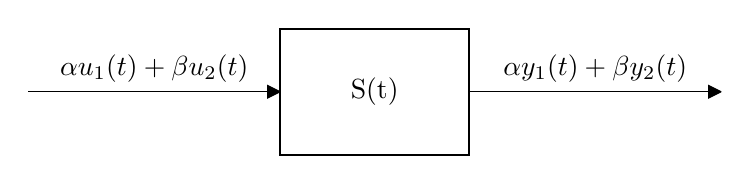
\begin{tikzpicture}[scale=0.8]
%\draw [lightgray](0,0) grid (11, 2);

\draw (0,1) -- (4,1);
\draw [fill]( 4,1) -- ( 3.8, 1.1) -- ( 3.8,0.9) -- ( 4,1);
\draw [black, thick](4,0) rectangle (7, 2) ; % S1 
\draw (7,1) -- (11,1);
\draw [fill]( 11,1) -- (10.8, 1.1) -- (10.8,0.9) -- (11,1);

\node [above] at (2,1){$\alpha u_1(t) + \beta u_2(t)$};
\node at ( 5.5, 1){S(t)};
\node [above] at (9,1){$\alpha y_1(t) + \beta y_2(t)$};

\end{tikzpicture}
\label{fig:principioSuperposicao}

{\small Fonte: \cite{Ogata}}
\end{figure}



%%%%%%%%%%%%%%%%%%%%%%%%%%%%%%%%%%%%%%%%%%%%%%%%%%%%%%%%%%%
\subsubsection{Linearização}
%%%%%%%%%%%%%%%%%%%%%%%%%%%%%%%%%%%%%%%%%%%%%%%%%%%%%%%%%%%

Para o processo de linearização de um sinal, uma forma comumente utilizada é através da Série de Taylor, onde dado um plano cartesiano e uma função \emph{f} com um ponto qualquer com coordenadas \emph{x} e \emph{y} com pequenas variações $\overline{x}$ e $\overline{y}$, temos que:

\begin{center}
\begin{equation}
y = \overline{y} + 
\frac{df}{dx} \left| \frac{ }{ } _{\overline{x}} \right. \, (x - \overline{x}) + 
\frac{1}{2!} \frac{d²f}{dx²} \left| \frac{ }{ } _{\overline{x}} \right. \, (x - \overline{x})² +
\frac{1}{3!} \frac{d³f}{dx³} \left| \frac{ }{ } _{\overline{x}} \right. \, (x - \overline{x})³ + ...
\label{eqn:SerieTaylor}
\end{equation}
\end{center}

A Série de Taylor é truncada após o segundo membro da somatória, pois $(x - \overline{x}^n )$ é cada vez menor na medida em que o expoente aumenta, fazendo com que tal parcela da somatória tenda a zero, assim despreza-se tais termos e tem-se:

\begin{center}
\begin{equation}
y = \overline{y} + 
\frac{df}{dx} \left| \frac{ }{ } _{\overline{x}} \right. \, (x - \overline{x})
\label{eqn:SerieTaylorTruncada}
\end{equation}
\end{center}



%%%%%%%%%%%%%%%%%%%%%%%%%%%%%%%%%%%%%%%%%%%%%%%%%%%%%%%%%%%
\subsection{Transformada de Laplace}
%%%%%%%%%%%%%%%%%%%%%%%%%%%%%%%%%%%%%%%%%%%%%%%%%%%%%%%%%%%
 
A Transformada de Laplace é utilizada em controle como uma ferramenta matemática para facilitar a solução de equações diferenciais lineares, utilizando uma variável complexa \emph{s}, operações como derivação e integração podem ser substituidas por operações algébricas no plano complexo, domínio da frequência, e após a resolução realiza-se a Transformada Inversa de Laplace para retornar a solução para o domínio do tempo.

A definição e sua dedução de forma rigorosa podem ser encontradas em \cite{Ogata} e não será discutida neste trabalho, mas vale aqui apresentar apenas a sua definição e uma parte da tabela de conversão.

A Transformada de Laplace é definida como:

\begin{equation}
\mathscr{L}\{f(t)\} = F(s) = \int_{0}^{\infty} f(t) e^{-st} dt
\label{eq:transfLaplace}
\end{equation} 

Onde:

\setlength{\parindent}{2cm}
$\mathscr{L}$ : Operador da Transformada de Laplace 

$f(t)$ : função da variável $t$ tal que $f(t) = 0$ para $t < 0$ 

$F(s)$ : Transformada de Laplace de $f(t)$

$s$ : variável complexa
\\

\setlength{\parindent}{0cm}
A Transformada Inversa de Laplace é definida como:

\begin{equation}
\mathscr{L}^{-1} \{F(s)\} =  \frac{1}{2 \pi j} \int_{c-j\infty}^{c+j\infty}F(s) e^{st} ds  \text{ , para } t > 0
\label{eq:transfInvLaplace}
\end{equation}

Onde:

\setlength{\parindent}{2cm}
$\mathscr{L}^{-1}$ : Operador da Transformada Inversa de Laplace

$c$ : Número real constante, abscissa da convergência.

\setlength{\parindent}{1cm}

Dificilmente a Transformada Inversa de Laplace é utilizada, podendo ser utilizado o método de frações parciais ou a tabela de conversão.

A Tabela \ref{tab:Laplace} mostra alguns pares de Transformadas de Laplace, e uma tabela mais completa pode ser encontrada no Capítulo 2 de \cite{Ogata}. 

\begin{table}[h]
\centering
\caption{Pares de Transformadas de Laplace}
\label{tab:Laplace}
\begin{tabular}{c|c}
\hline
$f(t)$ & $F(s)$ \\
\hline
\hline
Impulso unitário $\delta(t)$ 		& $1$ 			\\ \hline
Degrau unitário $1(t)$ 			& $\frac{1}{s}$		\\ \hline
$t$ 					& $\frac{1}{s^2}$ 	\\ \hline
$\frac{t^{n-1}}{(n-1)!} (n=1,2,3,...)$ 	& $\frac{1}{s^n}$ 	\\ \hline
$t^n (n=1,2,3,...)$ 			& $\frac{n!}{s^{n+1}}$ 	\\ \hline
$e^{-at}$ 				& $\frac{1}{s+a}$ 	\\ \hline
$t^n e^{-at} (n=1,2,3,...)$ 		& $\frac{n!}{(s+a)^{n+1}}$ \\\hline
$\frac{1}{a} (1-e^{-at})$ 		& $\frac{1}{s(s+a)}$ 	\\ \hline
$\frac{1}{b-a}(e^{-at}-e^{-bt})$ 	& $\frac{1}{(s+a)(s+b)}$ \\ \hline
\end{tabular}
\end{table}





%%%%%%%%%%%%%%%%%%%%%%%%%%%%%%%%%%%%%%%%%%%%%%%%%%%%%%%%%%%
\section{Ação de Controle}
%%%%%%%%%%%%%%%%%%%%%%%%%%%%%%%%%%%%%%%%%%%%%%%%%%%%%%%%%%%



A ação de controle é a forma como se busca atender os chamados requisitos de desempenho do sistema, 
que de um modo geral se efetuam através de modificações das características da relação entrada/saída para se obter os valores desejados dessa relação, 
ou ainda ajustar o comportamento da saída para uma dada entrada específica.


Os principais e mais comuns requisitos de desempenho dos sistemas são associados a velocidade de resposta, 
presença ou não de oscilações na estabilização e 
a exatidão da resposta do sistema em relação ao valor desejado, 
chamada de erro de regime estacionário.


O erro de regime estacionário, mostrada na Figura \ref{fig:funcaoResposta}, 
é uma medida que vai tender a zero em sistemas ideais, 
mas que na realidade não alcança o valor zero, 
assim assume-se um valor aceitável, 
5\% do valor da resposta desejada para sistemas não críticos e 
2\% para sistemas de maior grau de criticidade, 
para assumir que o sistema entrou em estabilidade, 
e a resposta real é aceita como tendo atingido o valor de resposta desejada. 



\begin{figure}[!htb]
\centering
\caption{Gráfico da função Resposta}
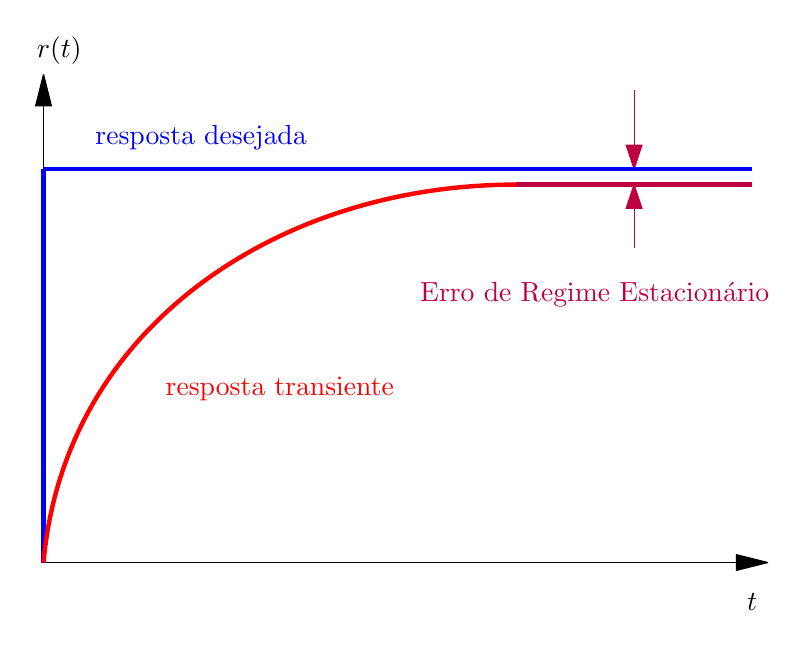
\begin{tikzpicture}[scale=1.00]
%\draw [lightgray, dashed](0,0) grid (8.8,5.8);

\draw [->] (0,0) -- (9,0); 
\draw [fill] (0,6.2) -- (-0.1, 5.8) -- (0.1,5.8) -- (0,6.2);

\draw [->] (0,0) -- (0,6);
\draw [fill] (9.2,0) -- (8.8,0.1) -- (8.8,-0.1)--(9.2,0.0);

\draw [purple, ->] (7.5,4.0) -- (7.5,4.6); 
\draw [purple, fill] (7.5,4.8) -- (7.4,4.5) -- (7.6,4.5)--(7.5,4.8);

\draw [purple, ->] (7.5,6.0) -- (7.5,5.2); 
\draw [purple, fill] (7.5,5.0) -- (7.4,5.3) -- (7.6,5.3)--(7.5,5.0);

\node at (9.0,-0.5) {$t$};
\node at (0.2,6.5) {$r(t)$};

\draw [blue, ultra thick] (0.0,5.0) -- (9.0,5.0);
\draw [blue, ultra thick] (0.0,0.0) -- (0.0,5.0);

\draw [red, ultra thick] (0,0) to [out=85, in=180] (6,4.8);

\draw [purple, ultra thick] (6,4.8) -- (9,4.8);

\node at (2.0,5.4)[blue]{{resposta desejada}};
\node at (3.0,2.2)[red]{{resposta transiente}};
\node at (7.0,3.4)[purple]{{Erro de Regime Estacionário}};

\end{tikzpicture} 
\label{fig:funcaoResposta}

{\small Fonte: \cite{dorf2011modern} }
\end{figure}




Para realizar o controle de um sistema é necessário que estejam bem definidos os seus requisitos, 
que são os objetivos a serem atendidos. 
Quando um sistema por si só já atende aos requisitos, 
não há a necessidade de controle. 
De forma oposta, é projetado o sistema de controle, 
que pode ser em malha aberta ou fechada, 
clássico ou moderno, convencional ou não-convencional, 
dependendo das características físicas do sistema. 


Para a execução de um sistema de controle podem ser verificados requisitos do sistema de duas formas básicas, 
sendo a primeira através dos testes e levantamento empírico da sua curva de resposta ou através de seu modelo matemático, 
quando trabalha-se com elementos já bem estudados e com a equação que representa seu comportamento empírico bem estabelecida por diversos estudos anteriores.


Em \citeauthor{dorf2011modern}(\citeyear{dorf2011modern}) 
%- Capítulo 7.6 - \emph{PID Controllers} 
é abordado o controlador PID, 
uma das principais soluções e a mais encontrada em aplicações industriais segundo \citeauthor{Ogata}(\citeyear{Ogata}), 
que trata do mesmo tema e as versões de PID modificados no Capítulo 10 de seu trabalho. 
Ações de controle do tipo PID são responsáveis por controlar a planta e atender aos requisitos de desempenho desejados ao sistema.





\newpage

O controle em malha aberta é o sistema mais simples de ser implementado, não possui realimentação, ou seja, o controlador não possui uma indicação da variável controlada, não sendo possível a sua correção caso haja alguma interferência, oscilação, ruído, ou mesmo que o sistema não apresente baixo rendimento.

\begin{figure}[!htb]
\centering
\caption{ Sistema de controle em malha aberta}
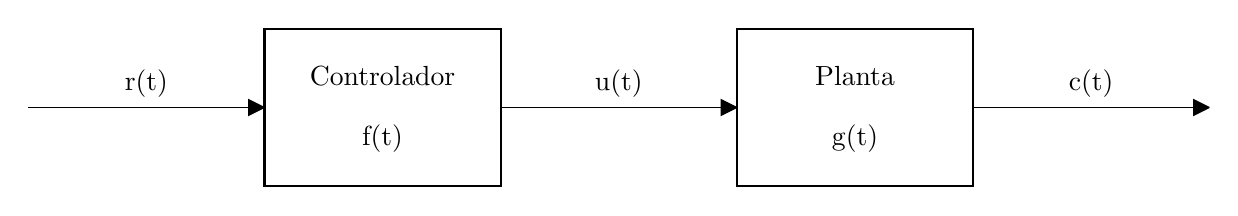
\begin{tikzpicture}[scale=1.0]
%\draw [lightgray](0,0) grid (15,2);
\draw (0,1) -- (3,1);
\draw [black, thick](3,0) rectangle (6, 2) ; 
\draw (6,1) -- (9,1);
\draw [black, thick](9,0) rectangle (12, 2) ; 
\draw (12,1) -- (15,1);

\draw [fill]( 3,1) -- ( 2.8, 1.1) -- ( 2.8,0.9) -- ( 3,1);
\draw [fill]( 9,1) -- ( 8.8, 1.1) -- ( 8.8,0.9) -- ( 9,1);
\draw [fill](15,1) -- (14.8, 1.1) -- (14.8,0.9) -- (15,1);

\node at ( 4.5, 1.4){Controlador};
\node at ( 4.5, 0.6){f(t)};
\node at (10.5, 1.4){Planta};
\node at (10.5, 0.6){g(t)};
\node [above] at ( 1.5,1){r(t)};
\node [above] at ( 7.5,1){u(t)};
\node [above] at (13.5,1){c(t)};
\end{tikzpicture}
\label{fig:AcaoMalhaAberta}

{\small Fonte: \cite{Ogata}}
\end{figure}

O sistema físico aqui estudado possui comportamento exponencial que pode ser descrito pela equação \ref{eq:ftSistOrdem1}. 




\begin{equation}
	 \frac{d c(t)}{dt} + c(t) = r(t) \rightarrow  \mathscr{L} \to \frac{C(s)}{R(s)} = \frac{K}{s + a} 
\label{eq:ftSistOrdem1}
\end{equation}

%\begin{equation}
%\therefore \frac{C(s)}{R(s)} = \frac{k}{s+a}
%\label{eq:ftSistOrdem1}
%\end{equation}

Onde:

\setlength{\parindent}{2cm}

$t$ : tempo,$ r(t) = 0$ , para t $<$ 0;

$\mathscr{L}$ : Operador de Laplace;

$c(t)$ : Variável controlada no domínio do tempo;

$C(s)$ : Variável controlada no domínio da frequência;

$r(t)$ : Valor de referência (\emph{setpoint}) no domínio do tempo;

$R(s)$ : Valor de referência (\emph{setpoint}) no domínio da frequência.

$K$ : Constantede proporcionalidade;

$s$ : Variável complexa de Laplace;

$a$ : Polo da função.
\setlength{\parindent}{1cm}

Sendo assim, para um estímulo de entrada do tipo \textbf{degrau}, conforme Tabela \ref{tab:Laplace}, com amplitude \textbf{A}, temos $ R(s) = \frac{A}{s}$ e aplicando a Transformada Inversa de Laplace:

\begin{equation}
C(s) = \frac{K}{s+a} \frac{A}{s} \rightarrow \mathscr{L}^{-1} \to c(t) = \frac{K A}{a} (1 - e^{-at})
\label{eq:degrauA}
\end{equation}

A Figura \ref{fig:degrauA} mostra um sinal do tipo degrau com amplitude \textbf{A} aplicado ao sistema de teste, que responde conforme um conforme um sistema de primeira ordem como mostrado na Figura \ref{fig:cRegime}. A partir de um determinado instante de tempo, entra em regime constante ($c_{reg}$), alcançando o valor de referência dado pelo degrau de amplitude A. Assim quando $ t \rightarrow \infty $  então $ c_{reg} \rightarrow A $:


\begin{figure}
\centering
\caption{Sistema de Primeira Ordem}
\subfloat[Sinal de entrada tipo degrau com amplitude A]{\label{fig:degrauA}
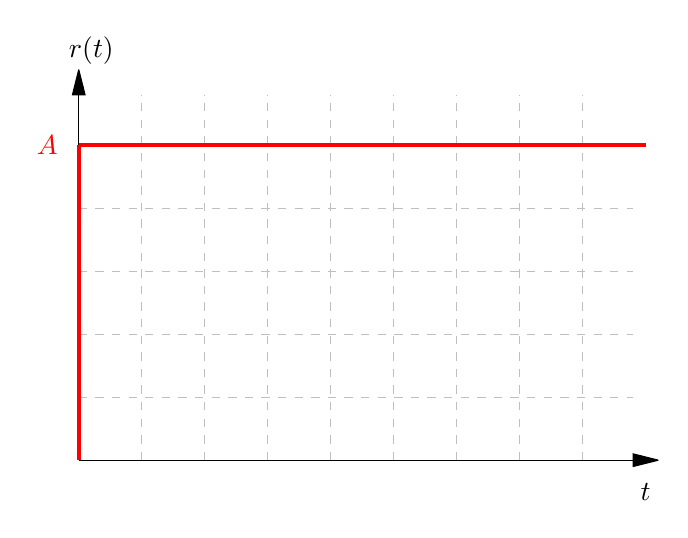
\begin{tikzpicture}[scale=0.8]
\draw [lightgray, dashed](0,0) grid (8.8,5.8);
\draw [->] (0,0) -- (9,0);
\draw [fill] (0,6.2) -- (-0.1, 5.8) -- (0.1,5.8) -- (0,6.2);
\draw [->] (0,0) -- (0,6);
\draw [fill] (9.2,0) -- (8.8,0.1) -- (8.8,-0.1)--(9.2,0.0);
\node at (9.0,-0.5) {$t$};
\node at (0.2,6.5) {$r(t)$};
\draw [red, ultra thick] (0.0,5.0) -- (9.0,5.0);
\draw [red, ultra thick] (0.0,0.0) -- (0.0,5.0);
\node at (-0.5,5.0)[red]{$A$};
\end{tikzpicture} }
\subfloat[Resposta transitória e regime de acomodação]{\label{fig:cRegime}
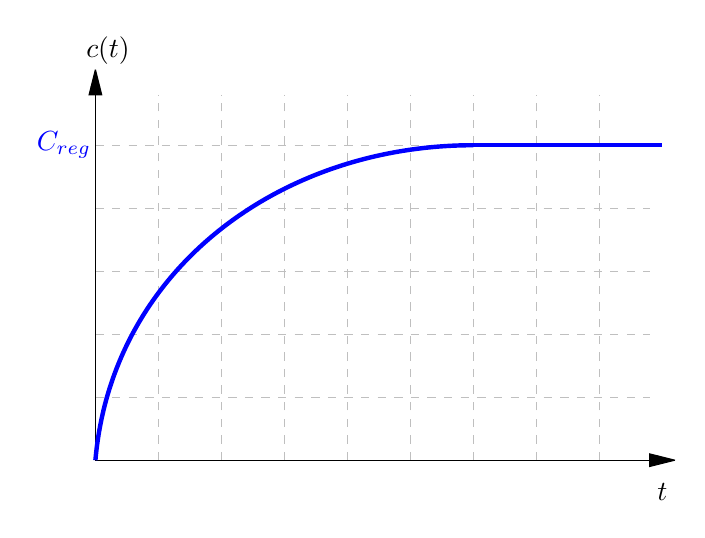
\begin{tikzpicture}[scale=0.8]
\draw [lightgray, dashed](0,0) grid (8.8,5.8);
\draw [->] (0,0) -- (9,0);
\draw [fill] (0,6.2) -- (-0.1, 5.8) -- (0.1,5.8) -- (0,6.2);
\draw [->] (0,0) -- (0,6);
\draw [fill] (9.2,0) -- (8.8,0.1) -- (8.8,-0.1)--(9.2,0.0);
\node at (9.0,-0.5) {$t$};
\node at (0.2,6.5) {$c(t)$};
\node at (-0.5,5.0)[blue]{$C_{reg}$};
\draw [blue, ultra thick] (0,0) to [out=85, in=180] (6,5);
\draw [blue, ultra thick] (6,5) -- (9,5);
\end{tikzpicture}}
\label{fig:sistPrimeiraOrdem}

{\small Fonte: \cite{Ogata}}
\end{figure}

%\begin{equation}
%c_{reg} = \lim_{t \rightarrow \infty} \frac{KA}{a}(1-e^{-at}) = \frac{KA}{a}
%\label{eq:cregime}
%\end{equation}

Aplicando o Teorema do Valor Final pode-se ver que o \emph{$c_{reg}$} estabiliza em um valor constante como mostrado pela Equação \ref{eq:teoremaValorFinal}:

\begin{equation}
C_{reg} = \lim_{s \rightarrow 0} sC(s) = \lim_{s \rightarrow 0} s\ \frac{K}{s+a}\frac{A}{s} = \frac{KA}{a}
\label{eq:teoremaValorFinal}
\end{equation}

Matematicamente, quanto maior o valor de \emph{t} na Equação \ref{eq:degrauA}, o resultado de sua exponenencial tende a zero, levando a um resultado que depende apenas das constantes, como mostrado na Equação \ref{eq:teoremaValorFinal}. 

Tomando $t= \frac{1}{a} = a^{-1} = \tau$ para gerar um valor conhecido em $e^{-at}$, da Equação \ref{eq:degrauA} temos:


\begin{equation}
c(a^-1) = \frac{KA}{a}(1-e^{-(a.a^{-1})}) = \frac{KA}{a}(1-e^{-1}) = \frac{KA}{a}.0,63 = 0,63 . C_{reg}
\end{equation}

A Figura \ref{fig:constTempo} mostra a constante de tempo $\tau$, que é atingida quando o sistema alcança 63\% do seu valor de regime. Como sabemos que $\tau = \frac{1}{a}$, então o polo do sistema, que leva o denominador da Equação \ref{eq:degrauA} a zero, é:

\begin{equation}
a = \frac{1}{\tau}
\end{equation}



\begin{figure}
\centering
\caption{Constante de tempo}
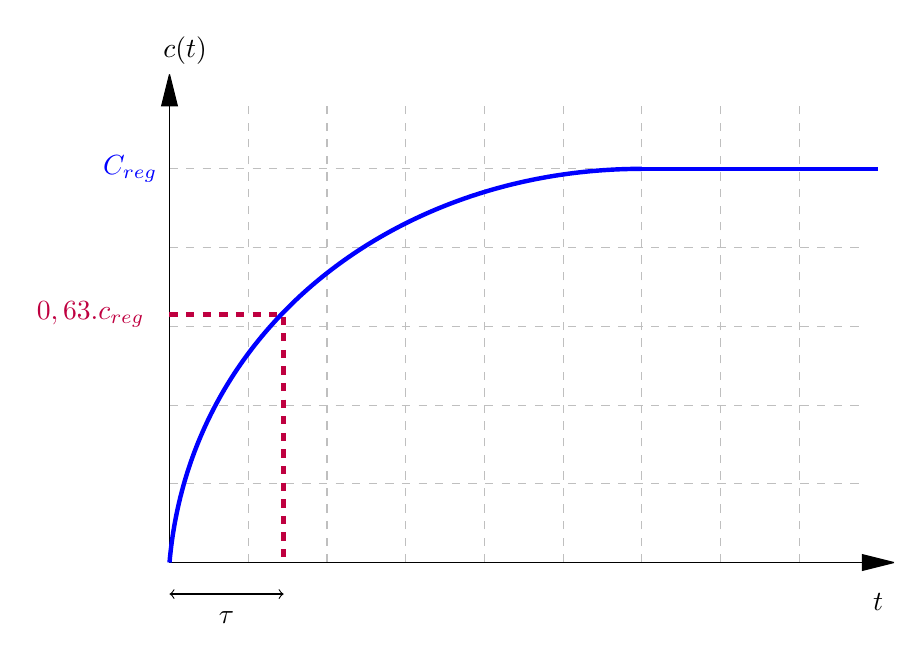
\begin{tikzpicture}[scale=1.0]
\draw [lightgray, dashed](0,0) grid (8.8,5.8);

\draw [->] (0,0) -- (9,0);
\draw [fill] (0,6.2) -- (-0.1, 5.8) -- (0.1,5.8) -- (0,6.2);
\draw [->] (0,0) -- (0,6);
\draw [fill] (9.2,0) -- (8.8,0.1) -- (8.8,-0.1)--(9.2,0.0);

\node at (9.0,-0.5) {$t$};
\node at (0.2,6.5) {$c(t)$};

\node at (-0.5,5.0)[blue]{$C_{reg}$};
\node at (-1,5.0*0.63)[purple]{$0,63.c_{reg}$};
\draw [purple, ultra thick, dashed] (0.0,5.0*0.63) -- (1.45,5.0*0.63)
						   -- (1.45,0.0);
\draw [blue, ultra thick] (0,0) to [out=85, in=180] (6,5);
\draw [blue, ultra thick] (6,5) -- (9,5);

\draw [<->] (0.0,-0.4) -- (1.45,-0.4); 
\node at (1.45/2,-0.7){$\tau$};

\end{tikzpicture}
\label{fig:constTempo}

{\small Fonte: \cite{Ogata}}
\end{figure}

Portanto:

\begin{equation}
K = \frac{ac_{reg}}{A}
\label{eq:calcK}
\end{equation}

%\begin{tikzpicture}
%\begin{axis}
%\addplot[title=Gráfico de uma função, 
%	xlabel = {$x$}, ylabel={$y$},
% 	red!70!blue, very thick, samples=200,
%	domain=-3:3]{x/(x^4-3*x^2+4)};
%\end{axis}
%\end{tikzpicture}


\subsection{ Duas posições ou Liga-Desliga }
É o tipo de ação de controle mais simples de ser implementado, porém o de menor precisão, pois opera com potência máxima até que o sensor atinja um determinado valor limite, mudando a ação para potência mínima, geralmente zero.

\begin{figure}[!htb]
\centering
\caption{Ação de Controle Liga-Desliga}
\center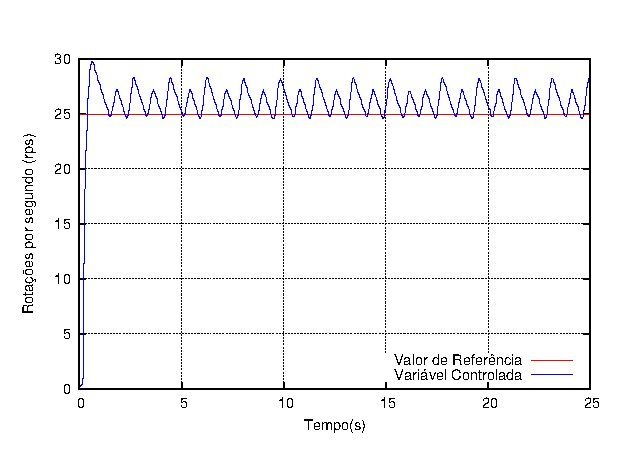
\includegraphics[scale=1]{./imagens/acaoControle-ligaDesliga.eps}
\label{fig:acaoControleLigaDesliga}

{\small Fonte: Próprio autor}
\end{figure}

A Figura \ref{fig:acaoControleLigaDesliga} mostra o gráfico obtido no sistema de teste, onde a velocidade de rotação do motor oscila entre os valores de 25 e 30 rps, sendo o valor desejado em 25 rps. 
Todas estas oscilações podem representar perda de energia, pois o motor está recebendo energia em excesso sem necessidade, porém sua implementação é simples e não requer um conhecimento específico e aprofundado de controle.


%
%\begin{figure}[!htb]
%\centering
%\caption{Código da Ação de Controle Liga-Desliga}
%\begin{minipage}{0.8\linewidth}
%\begin{lstlisting}
%long controlador_LigaDesliga{ long setpoint, long sensor }
%{
%  if( sensor > setpoint }
%    return( 0 );
%  else
%    return( 100 );
%}
%\end{lstlisting}
%\end{minipage}
%\label{fig:codigoAcaoLigaDesliga}

%{\small Fonte: Próprio autor}
%\end{figure}

%O código fonte que gerou o resultado obtido na Figura \ref{fig:acaoControleLigaDesliga} é  mostrado na Figura \ref{fig:codigoAcaoLigaDesliga}, sendo apresentada apenas a função que realiza função de controle, que neste caso tem como parâmetros de entrada os valores de \textit{\texttt{setpoint}} e do \textit{\texttt{sensor}} e o seu valor de retorno é o parâmetro de entrada da função de acionamento da modulação por largura de pulso (\textit{PWM - Pulse Width Modulation}), que neste caso utiliza apenas os valores extremos.



\subsection{ Controlador Proporcional (P) } 

 No controle proporcional, 
o erro é multiplicado por uma constante \emph{kp} 
gerando o sinal \emph{u\{t\}}, 
que é a variável manipulada que atua sobre o 
sistema \emph{g(t)}.

\begin{equation}
 u(t) = kp . e(t)
\label{eq:acaoP}
\end{equation}


O diagrama de blocos da Figura \ref{fig:malhaFechadaP} mostra o bloco \emph{kp} que tem seu comportamento descrito pela Equação \ref{eq:acaoP} e que atua diretamente sobre o sistema através da variável manipulada $u(t)$.

\begin{figure}[!htb]
\centering
\caption{ Diagrama em blocos de sistema de controle em malha fechada utilizando notação matemática}
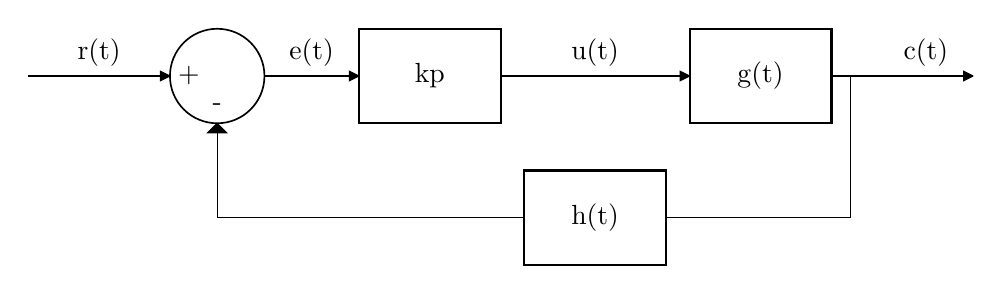
\begin{tikzpicture}[scale=0.6]
%\draw [lightgray](-3,0) grid (17, 2);
%\draw [lightgray](-3,0) grid (17,-3);
%\draw [semithick,red] (0,0) circle (0.1);

\draw (-3,1) -- (0,1);
\draw [fill]( 0,1) -- (-0.2, 1.1) -- ( -0.2,0.9) -- (0,1);
\draw [semithick,black] (1,1) circle (1.0); % Somador
\draw (2.0,1) -- (4,1);
\draw [fill]( 4,1) -- ( 3.8, 1.1) -- ( 3.8,0.9) -- ( 4,1);
\draw [black, thick](4,0) rectangle (7, 2) ; % Controlador 
\draw (7,1) -- (11,1);
\draw [fill]( 11,1) -- (10.8, 1.1) -- (10.8,0.9) -- (11,1);
\draw [black, thick](11,0) rectangle (14, 2) ; % Planta
\draw (14,1) -- (17,1);
\draw [fill](17,1) -- (16.8, 1.1) -- (16.8,0.9) -- (17,1);

\draw [black, thick](7.5,-1) rectangle (10.5, -3) ; % Sensor
\draw (14.4, 1) -- (14.4, -2) -- (10.5,-2);
\draw ( 7.5,-2) -- ( 1, -2) -- (1,0);
\draw [fill](1,0) -- (1.2,-0.2) -- (0.8,-0.2) -- (1,0);

\node [above] at (-1.5,1){r(t)};
\node at (0.4,1){+};
\node at (1,0.4){-};
\node [above] at (3.0,1){e(t)};
\node at ( 5.5, 1){kp};
\node [above] at (9.0,1){u(t)};
\node at (12.5, 1){g(t)};
\node [above] at (16.0,1){c(t)};
\node at ( 9.0,-2){h(t)};

\end{tikzpicture}
\label{fig:malhaFechadaP}

{\small Fonte: Próprio autor}
\end{figure}

Variando o valor de $kp$ pode-se ver pela Figura \ref{fig:acaoP} que quanto maior o seu valor, mais rápida é a resposta do sistema, ou seja, menor é o tempo necessário para alcançar o valor de referência, porém, depois de um determinado valor, o sistema apresenta um sobressinal, que pode ou não ser tolerável, dependendo das exigências da aplicação.

\begin{figure}[!htb]
\centering
\caption{Ação de Controle Proporcional}
\center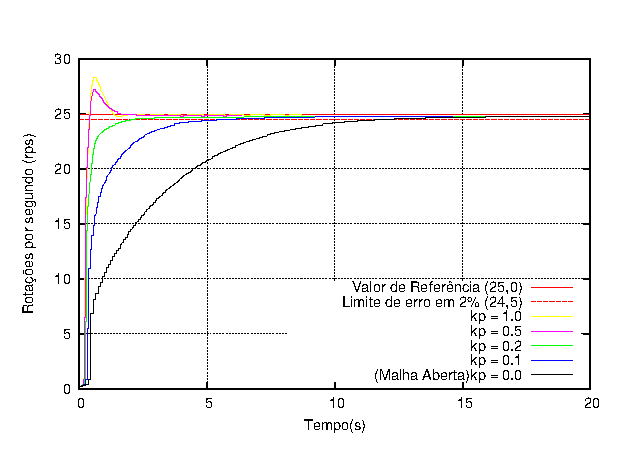
\includegraphics[scale=1.4]{./imagens/acaoP.eps}
\label{fig:acaoP}

{\small Fonte: Próprio autor}
\end{figure}

%O controlador que foi implementada a função proporcional está apresentado na Figura \ref{fig:codigoControladorP}, onde pode-se verificar a utilização de variáveis do tipo ponto flutuante (\emph{float}) para obtenção de maior precisão nos cálculos e consequantemente, no controle. O nome das variáveis faz alusão a sua representação no diagrama de blocos da Figura \ref{fig:malhaFechadaP}.

%A função implementada, declarada na linha 7 possui três parâmetros de entrada e possui um parâmetro de retorno, sendo:
%\begin{itemize}
%  \item $setpoint$ : recebe o valor de rotação desejado ao sistema, o valor de referência;
%  \item $max$ : representa o máximo valor que o sistema alcança;
%  \item $sensor$ : recebe o valor de rotação atual da planta;
%  \item $return $ : Parâmetro de retorno da função que assume um valor entre 0 e 100, pois é o parâmetro de entrada do controlador PWM que efetua o acionamento do motor.

%\end{itemize}



%\begin{figure}[!htb]
%\centering
%\caption{Código da Ação de Controle Proporcional}
%\begin{minipage}{0.8\linewidth}
%\lstset{firstnumber=1}
%\begin{lstlisting}
%float kp = 0.1;
%float ki = 0.0002;
%float kd = 2.0;
%float yT, rT, eT, iT, dT, uT;
%long  Cout, pwmAlvo;

%long controlador{ long setpoint, long max, long sensor }
%{
%    rT = (float) setpoint;
%    yT = (float) sensor;
%    pwmAlvo = ((setpoint*100)/max);

    
%    eT = rT - yT;
    
%    uT = kp*eT;

%    Cout = pwmAlvo + uT;

%    if( Cout < 0 )
%        Cout = 0;
%    else if( Cout >= 100 )
%        Cout = 100;

%    return( Cout );
%}
%\end{lstlisting}
%\end{minipage}
%\label{fig:codigoControladorP}

%{\small Fonte: Próprio autor}
%\end{figure}


%Nas linhas 9 e 10 os parâmetros de entradas são convertidos em ponto flutuante para realização dos cálculos e atribuidos às respectivas variáveis auxiliares.

%A variável \emph{pwmAlvo} recebe o valor percentual da velocidade de referência, como a velocidade mínima é zero, basta dividir o \emph{setpoint} pelo valor \emph{max} e multiplicar por \emph{100} conforme feito na linha 11.


%A linha 14 realiza o cálculo do erro, subtraindo do valor de referência (\emph{rT}) o valor do erro (\emph{ht}).

%Na linha 18 a variável manipilada recebe o erro (\emph{eT}) sendo multiplicado proporcionalmente pelo coeficiente kp, que caracteriza esta configuração de controle.

%A variável \emph{Cout}, é a variável com o valor que será o retorno da função, que serve de parâmetro de entrada ao gerador de sinal PWM que atua sobre o motor.

%\emph{Cout} recebe o valor da variável \emph{pwmAlvo} que é a aplicação de um degrau com valor de referência do sistema somado somada a \emph{uT} que possui o valor proporcional ao erro do sistema. 

%Inicialmente, considerando o sistema em repouso, o erro possui um valor alto, então, Cout é inicializada com um valor bem maior do que o necessário para gerar o valor de referência, ou seja, um valor de pwm referente a uma velocidade bem maior do que os \emph{25 rps} de referência da aquisição mostrada na Figura \ref{fig:acaoP}. Conforme o sistema começa a girar, e a velocidade aumenta, o erro diminui, o que diminui o incremento ao \emph{pwmAlvo}, até que este incremento seja zero quando o valor lido pelo sensor alcançar o valor de referência, que é o próprio valor do degrau que está em \emph{pwmAlvo}.

%O código entre as linhas 20 e 23 são necessárias apenas para não gerar um valor incorreto para o parâmetro do PWM, o que poderia causar falhas no acionamento. 










\subsection{ Controlador Integral (I) }

O controlador integral atua acumulando o erro do sistema, conforme equação descrita abaixo:


\begin{equation}
u(t) = ki \int_{0}^{\infty} e(t) dt
\end{equation}

A resposta apresentada pelo sistema está plotada na Figura \ref{fig:acaoI} e mostra que ao aumentar o valor do coeficiente \emph{ki} o sistema começou a oscilar e demorou mais para estabilizar dentro de um valor limite próximo ao valor de referência. 

\begin{figure}[!h]
\centering
\caption{Ação de Controle Integral}
\center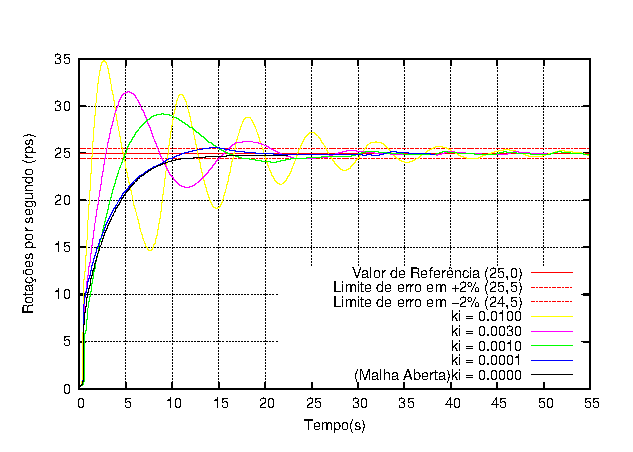
\includegraphics[scale=1.3]{./imagens/acaoI.eps}
\label{fig:acaoI}

{\small Fonte: Próprio autor}
\end{figure}

%A Figura \ref{fig:codigoControladorI} mostra o código da função que implementou o controlador com ação integral, responsáveis por gerar propriamente a ação de integração do erro.


%\begin{figure}[!htb]
%\centering
%\caption{Código da Ação de Controle Integral}
%\begin{minipage}{0.8\linewidth}
%\lstset{firstnumber=13}
%\begin{lstlisting}

%    eT = rT - yT;
%    iT += eT * i; 
%    uT = iT;
%\end{lstlisting}
%\end{minipage}
%\label{fig:codigoControladorI}

%{\small Fonte: Próprio autor}
%\end{figure}

A ação de integração é uma somatória de pequenas amostras do erro, que somadas ao longo do tempo levam o sistema a um erro zero, porém demoram mais tempo para alcançar a estabilidade e facilmente geram sobressinal.










\subsection{ Controlador Proporcional + Integral (PI) }

O controlador Proporcional Integral (PI) como o próprio nome indica, é a união das ações de controle que levam seu nome, e busca unir as suas propriedades.
 
\begin{equation}
u(t) = kp.e(t) + ki \int_{0}^{\infty} e(t) dt
\end{equation}


O intuito neste controlador é reduzir o tempo de resposta do sistema pelo controle proporcional e ao mesmo tempo gerar um erro nulo quando a estabilidade é atingida.





\begin{figure}[!htb]
\centering
\caption{ Diagrama em blocos de sistema de controle em malha fechada utilizando notação matemática}
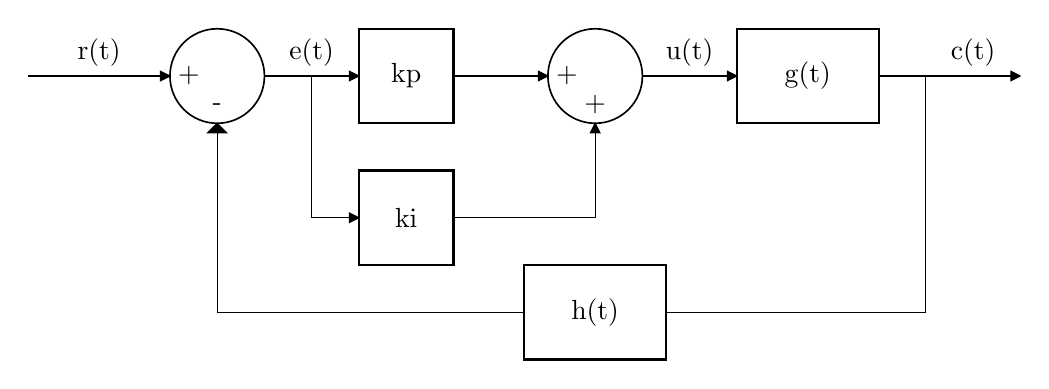
\begin{tikzpicture}[scale=0.6]

%\draw [lightgray](-3,0) grid (18, 2);
%\draw [lightgray](-3,0) grid (18,-5);
%\draw [semithick,red] (0,0) circle (0.1);

\draw (-3,1) -- (0,1);
\draw [fill]( 0,1) -- (-0.2, 1.1) -- ( -0.2,0.9) -- (0,1);
\draw [semithick,black] (1,1) circle (1.0); % Somador
\draw (2.0,1) -- (4,1);
\draw [fill]( 4,1) -- ( 3.8, 1.1) -- ( 3.8,0.9) -- ( 4,1);
\draw [black, thick](4,0) rectangle (6, 2) ; % Controlador P 
\draw (6,1) -- (8,1);
\draw [fill]( 8,1) -- (7.8, 1.1) -- ( 7.8,0.9) -- (8,1);
\draw [semithick,black] (9,1) circle (1.0); % Somador 2
\draw (10.0,1) -- (12,1);
\draw [fill]( 12,1) -- (11.8, 1.1) -- (11.8,0.9) -- (12,1);
\draw [black, thick](12,0) rectangle (15, 2) ; % Planta
\draw (15,1) -- (18,1);
\draw [fill](18,1) -- (17.8, 1.1) -- (17.8,0.9) -- (18,1);

\draw (3,1) -- (3,-2) -- (4,-2);
\draw [fill](4,-2) -- (3.8, -2.1) -- (3.8,-1.9) -- (4,-2);
\draw [black, thick](4,-1) rectangle (6,-3) ; % Controlador I
\draw (6,-2) -- (9,-2) -- (9,0);
\draw [fill](9,0) -- (8.9, -0.2) -- (9.1,-0.2) -- (9,0);



\draw [black, thick](7.5,-3) rectangle (10.5, -5) ; % Sensor
\draw (16, 1) -- (16, -4) -- (10.5,-4);
\draw ( 7.5,-4) -- ( 1, -4) -- (1,0);
\draw [fill](1,0) -- (1.2,-0.2) -- (0.8,-0.2) -- (1,0);

\node [above] at (-1.5,1){r(t)};
\node at (0.4,1){+};
\node at (1,0.4){-};
\node [above] at (3.0,1){e(t)};
\node at ( 5.0, 1){kp};
\node at (5.0,-2) {ki};
\node at (8.4,1){+};
\node at (9,0.4){+};
\node [above] at (11.0,1){u(t)};
\node at (13.5, 1){g(t)};
\node [above] at (17.0,1){c(t)};
\node at ( 9.0,-4){h(t)};

\end{tikzpicture}
\label{fig:malhaFechadaPI}

{\small Fonte: Próprio autor}
\end{figure}

Variando o valor de $kp$ pode-se ver pela Figura \ref{fig:acaoP} que quanto maior o seu valor, mais rápida é a resposta do sistema, ou seja, menor é o tempo necessário para alcançar o valor de referência, porém, depois de um determinado valor, o sistema apresenta um sobressinal, que pode ou não ser tolerável, dependendo das exigências da aplicação.

%\begin{figure}[!htb]
%\centering
%\caption{Ação de Controle Proporcional}
%\center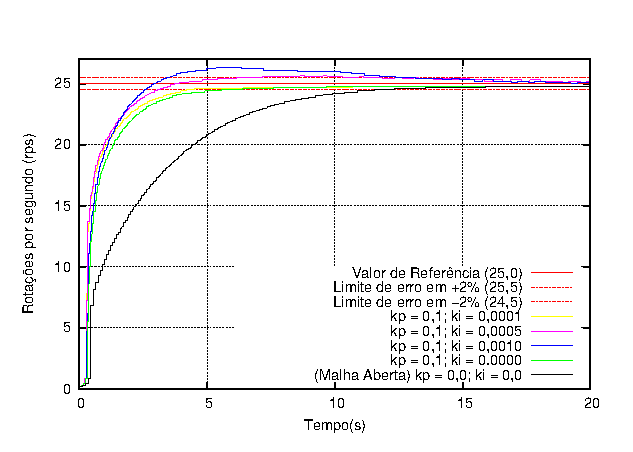
\includegraphics[scale=1.4]{./imagens/acaoPI.eps}
%\label{fig:acaoP}

%{\small Fonte: Próprio autor}
%\end{figure}






\begin{figure}[!htb]
\caption{Ação de Controle Proporcional Integral}
\center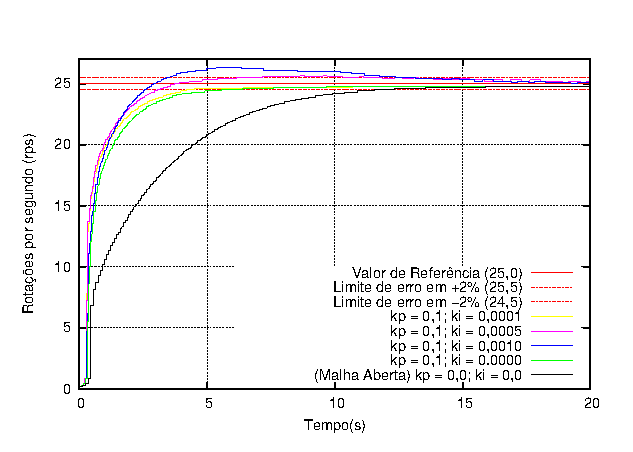
\includegraphics[scale=1.2]{./imagens/acaoPI.eps}
\label{fig:acaoPI}

{\small Fonte: Próprio autor}
\end{figure}

Como pode-se ver no gráfico da Figura \ref{fig:acaoPI} foi utilizado um valor de $ki = 0.1$ para obter uma subida em um tempo tido como bom, ou seja, subida mais rápida e sem gerar sobressinal, de acordo com os valores mostrados na Figura \ref{fig:acaoP}.





%\begin{figure}[!htb]
%\centering
%\caption{Código da Ação de Controle Proporcional Integral}
%\begin{minipage}{0.8\linewidth}
%\lstset{firstnumber=13}
%\begin{lstlisting}

%    eT = rT - yT;
%    iT += eT * i; 
%    uT = iT + p*eT;
%\end{lstlisting}
%\end{minipage}
%\label{fig:codigoControladorPI}

%{\small Fonte: Próprio autor}
%\end{figure}

%O código da Figura \ref{fig:codigoControladorPI} mostra a implementação das funções de controle proporcional e integral, sendo que a linha 15 mostra a somatória característica do controle integral.










%\subsection{ Controlador Proporcional + Derivativo (PD) }

%A ação de controle proporcional e derivativo propicia uma resposta mais rápida, pois a ação derivativa gera um grande erro se houver variações abruptas.

%\begin{equation}
%u(t) = kp.e(t) + kd. \frac{d e(t)}{dt}
%\end{equation}

%A figura \ref{fig:acaoPD} mostra que a resposta do sistema é a mais rápida dos ações de controle estudadas, e também gera o maior sobressinal. 


%\begin{figure}[!htb]
%\centering
%\caption{Ação de Controle Proporcional Derivativo}
%\center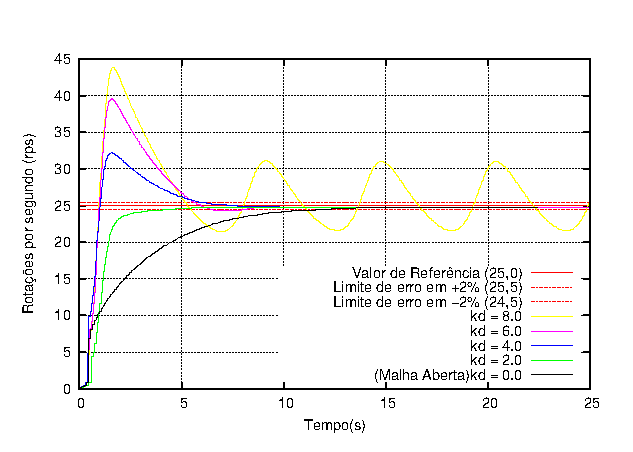
\includegraphics[scale=1.1]{./imagens/acaoPD.eps}
%\label{fig:acaoPD}

%{\small Fonte: Próprio autor}
%\end{figure}

% A linha 13 da Figura \ref{fig:codigoControladorPD} mostra como foi codificada a ação de controle Derivativa modificada.

%\begin{figure}[!htb]
%\centering
%\caption{Código da Ação de Controle Proporcional Derivativo}
%\begin{minipage}{0.8\linewidth}
%\lstset{firstnumber=13}
%\begin{lstlisting}
%    dT = (eT - (rT-yT)) * d;
%    eT = rT - yT;
%
%    uT = dT + p*eT;
%\end{lstlisting}
%\end{minipage}
%\label{fig:codigoControladorPD}

%{\small Fonte: Próprio autor}
%\end{figure}

%A ação de controle derivativa (PD) é modificada pois é utilizada a diferença do erro na iteração anterior com o erro com os dados atuais, diferente do que ocorre com o controlador PD teórico, onde a derivada implica na diferença entre o valor atual e uma pequena variação positiva do tempo, ou seja, uma amostra futura, que é impossível de ser obtida na pratica. 










%\subsection{ Controlador Proporcional + Integral + Derivativo (PID) }

%O controlador Proporcional Integral Derivativo é uma das configurações mais utilizadas por sua versatilidade, unindo as características que permitem ajustar o tempo de subida, o sobressinal e o erro de estado estacionário, conforme a necessidade e a aplicação.

%\begin{equation}
%u(t) = kp.e(t) + ki \int_{0}^{\infty} e(t) dt + kd. \frac{d e(t)}{dt}
%\end{equation}

%O controlador PID pode ser implementado de diversas formas, pode ter o parâmetro proporcional influenciando diretamente as demais ações, ou não, como neste caso onde as ações de controle são utilizadas de forma independentes, e o erro é utilizado para cada uma das partes da soma do sinal da variável manipulada ($u(t)$).

%\begin{figure}[!htb]
%\centering
%\caption{Ação de Controle Proporcional Integral Derivativo}
%\center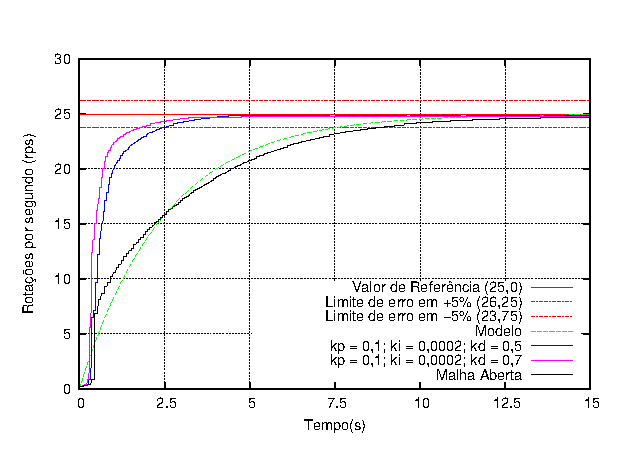
\includegraphics[scale=1.4]{./imagens/acaoPID.eps}
%\label{fig:acaoPID}

%{\small Fonte: Próprio autor}
%\end{figure}

%Os dois sinais utilizando o controle PID utilizou parâmetros já testados nos controladores anteriores para obter um resultado desejado, onde o sistema responde de forma bem rápida ao estímulo de entrada, tendo um tempo de subida entre 3 e 4 segundos para atingir a estabilidade com erro de estado estacionário menor do que 2\%, sem gerar sobressinal.


%Em comparação ao sinal de controle em malha aberta, que a estabilidade é alcançada em um tempo de aproximadamente 12 segundos, o ganho de velocidade é consideravel para o sistema estudado, pois foi reduzido a pelo menos um terço do tempo original.

%A Figura \ref{fig:codigoControladorPID} mostra a codificação completa dos parâmetros do PID, onde pode-se perceber que sua implementação é simples, apesar da teoria ser complexa. 

%\begin{figure}[!htb]
%\centering
%\caption{Código da Ação de Controle Proporcional Integral Derivativo}
%\begin{minipage}{0.8\linewidth}
%\lstset{firstnumber=13}
%\begin{lstlisting}
%    dT = (eT - (rT-yT)) * d;
%    eT = rT - yT;
%    iT += eT * i; 
%    uT = p*eT + iT + dT;
%\end{lstlisting}
%\end{minipage}
%\label{fig:codigoControladorPID}

%{\small Fonte: Próprio autor}
%\end{figure}


%Para o microcontrolador efetuar as subtrações é algo que requer pouco processamento, mas as multiplicações são bem mais complexas e exigem mais memória e tempo de processamento, e é claro que trabalhando em ponto flutuante esta complexidade também é muito grande. O controlador utilizado possui uma unidade de processamento de ponto flutuante, o que possibilitou uma performance capaz de efetuar todos os cálculos sem afetar a leitura de velocidade do sistema.


%%%%%%%%%%%%%%%%%%%%%%%%%%%%%%%%%%%%%%%%%%%%%%%%%%%%%%%%%%%
\section{Requisitos de desempenho do sistema}
%%%%%%%%%%%%%%%%%%%%%%%%%%%%%%%%%%%%%%%%%%%%%%%%%%%%%%%%%%%

Os sistemas de controle buscam atender os chamados requisitos de desempenho do sistema, que de um modo geral se efetuam através de modificações das características da relação entrada/saída para se obter os valores desejados dessa relação, ou ainda ajustar o comportamento da saída para uma dada entrada específica.

Os principais e mais comuns requisitos de desempenho dos sistemas são associados a velocidade de resposta, presença ou não de oscilações e a exatidão da resposta do sistema em relação ao valor desejado, chamada de erro de regime estacionário.

O erro de regime estacionário, mostrada na Figura \ref{fig:funcaoResposta}, é uma medida que vai tender a zero em sistemas ideais, mas que na realidade não alcança o valor zero, assim assume-se um valor aceitável, 5\% do valor da resposta desejada para sistemas não críticos e 2\% para sistemas de maior grau de criticidade, para assumir que o sistema entrou em estabilidade, e a resposta real é aceita como tendo atingido o valor de resposta desejada. 

\begin{figure}[!htb]
\centering
\caption{Gráfico da função Resposta}
\center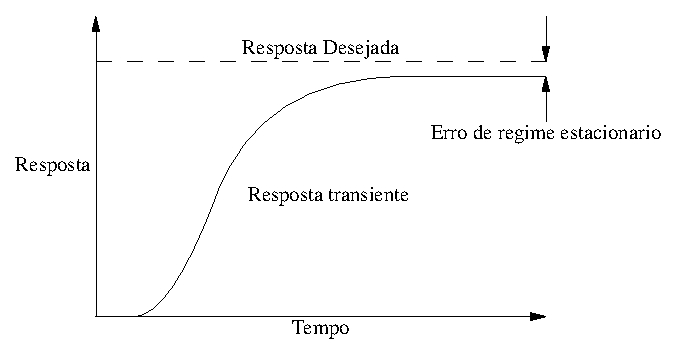
\includegraphics[scale=1]{./imagens/C400grafico.eps}
\label{fig:funcaoResposta}

{\small Fonte: Próprio autor}
\end{figure}

Para realizar o controle de um sistema é necessário que estejam bem definidos os seus requisitos, que são os objetivos a serem atendidos. Quando um sistema por si só já atende aos requisitos, não há a necessidade de controle. De forma oposta, é projetado o sistema de controle, que pode ser em malha aberta ou fechada, clássico ou moderno dependendo das características físicas do sistema. 

Para a execução de um sistema de controle podem ser verificados requisitos do sistema de duas formas básicas, sendo a primeira através dos testes e levantamento empírico da sua curva de resposta ou através de seu modelo matemático, quando trabalha-se com elementos já bem estudados e com a equação que representa seu comportamento empírico bem estabelecida por diversos estudos anteriores.



\newpage


